\Exercise El vector $\overrightarrow{PQ}=(3,-6)$ té l'extrem en el punt $Q(2,1)$. Determina les coordenades de l'origen $P$ i el mòdul d'aquest vector.

\Answer

Podem expressar el vector $\overrightarrow{PQ}$ com la diferència dels vectors que identifiquen els seus dos extrems:

\begin{minipage}{0.49\linewidth}
\[\overrightarrow{PQ}=Q-P\]
\begin{eqnarray*}
  (3,-6)&=&(2,1)-P\\
  P=&=&(2,1)-(3,-6)\\
  P&=&(-1,7)
\end{eqnarray*}
Pel que fa al mòdul:
\[\abs{\overrightarrow{PQ}}=\sqrt{3^2+(-6)^2}=\sqrt{45}=3\sqrt{5}\]
\end{minipage}
\hspace{0.01\linewidth}
\begin{minipage}{0.49\linewidth}
\begin{center}
  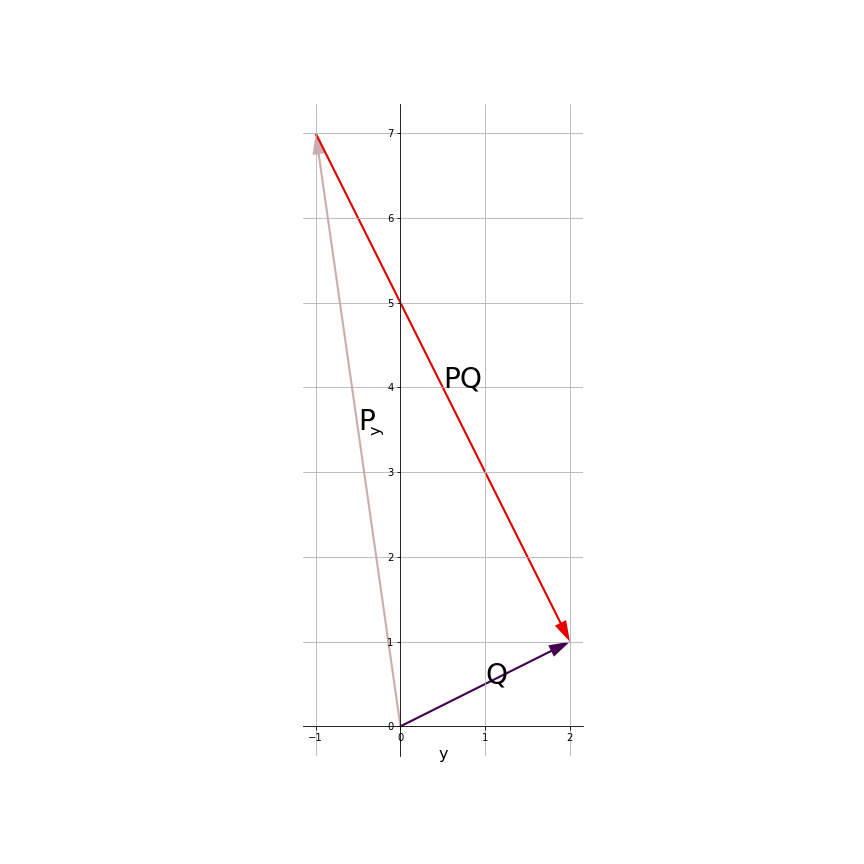
\includegraphics[scale=0.3]{vectorPQ2}
\end{center}
\end{minipage}


\blacksquare 